\subsection{Chính sách gửi thích ứng}\label{sec:03-system-implementation}
Ứng dụng đo throughput qua \texttt{/probe}, endpoint khoảng 64 KiB. Ngân sách probe ở chính sách gửi là 6 giây và có thể dùng số byte đọc một phần để ước lượng. Cấu hình hiện tại dùng ngưỡng mạng mạnh 1.000 kbit/s, mức còn phù hợp ảnh nén 50 kbit/s và confidence cao 0,90.

\begin{table}[htbp]\centering\small
\caption{Chính sách chọn chế độ gửi trong mã hiện tại}\label{tab:send-policy}
\begin{tabularx}{\textwidth}{P{.36\textwidth}X}
\toprule Điều kiện & Chế độ được chọn \\\midrule
Không có data & Thử SMS; nếu không gửi được thì giữ hàng đợi \\
Từ 1.000 kbit/s, confidence dưới 0,90 & Ảnh gốc và thông tin \\
Từ 1.000 kbit/s, confidence từ 0,90 & Chỉ thông tin khi cờ ưu tiên metadata bật \\
Từ 50 đến dưới 1.000 kbit/s & Ảnh nén và thông tin \\
Có data nhưng dưới 50 kbit/s & Chỉ thông tin \\
\bottomrule\end{tabularx}
\end{table}

Trong chế độ nén, ứng dụng dùng JPEG quality 60 với tham số \texttt{minWidth} và \texttt{minHeight} đều bằng 1.024 pixel. Khi ảnh đủ lớn, thư viện giữ tỷ lệ khung hình và giảm cạnh ngắn về 1.024 pixel; ảnh nhỏ không được phóng to. Cạnh dài có thể lớn hơn 1.024 pixel. Ảnh định dạng không phù hợp endpoint có thể được đổi sang JPEG. Cơ chế này giảm lượng dữ liệu ảnh cần truyền trong điều kiện mạng hạn chế.

Hình~\ref{fig:flow-adaptive-send} tổng hợp các nhánh quyết định chế độ gửi theo thông lượng mạng và độ tin cậy AI.

\begin{reportlandscapefigure}
\centering

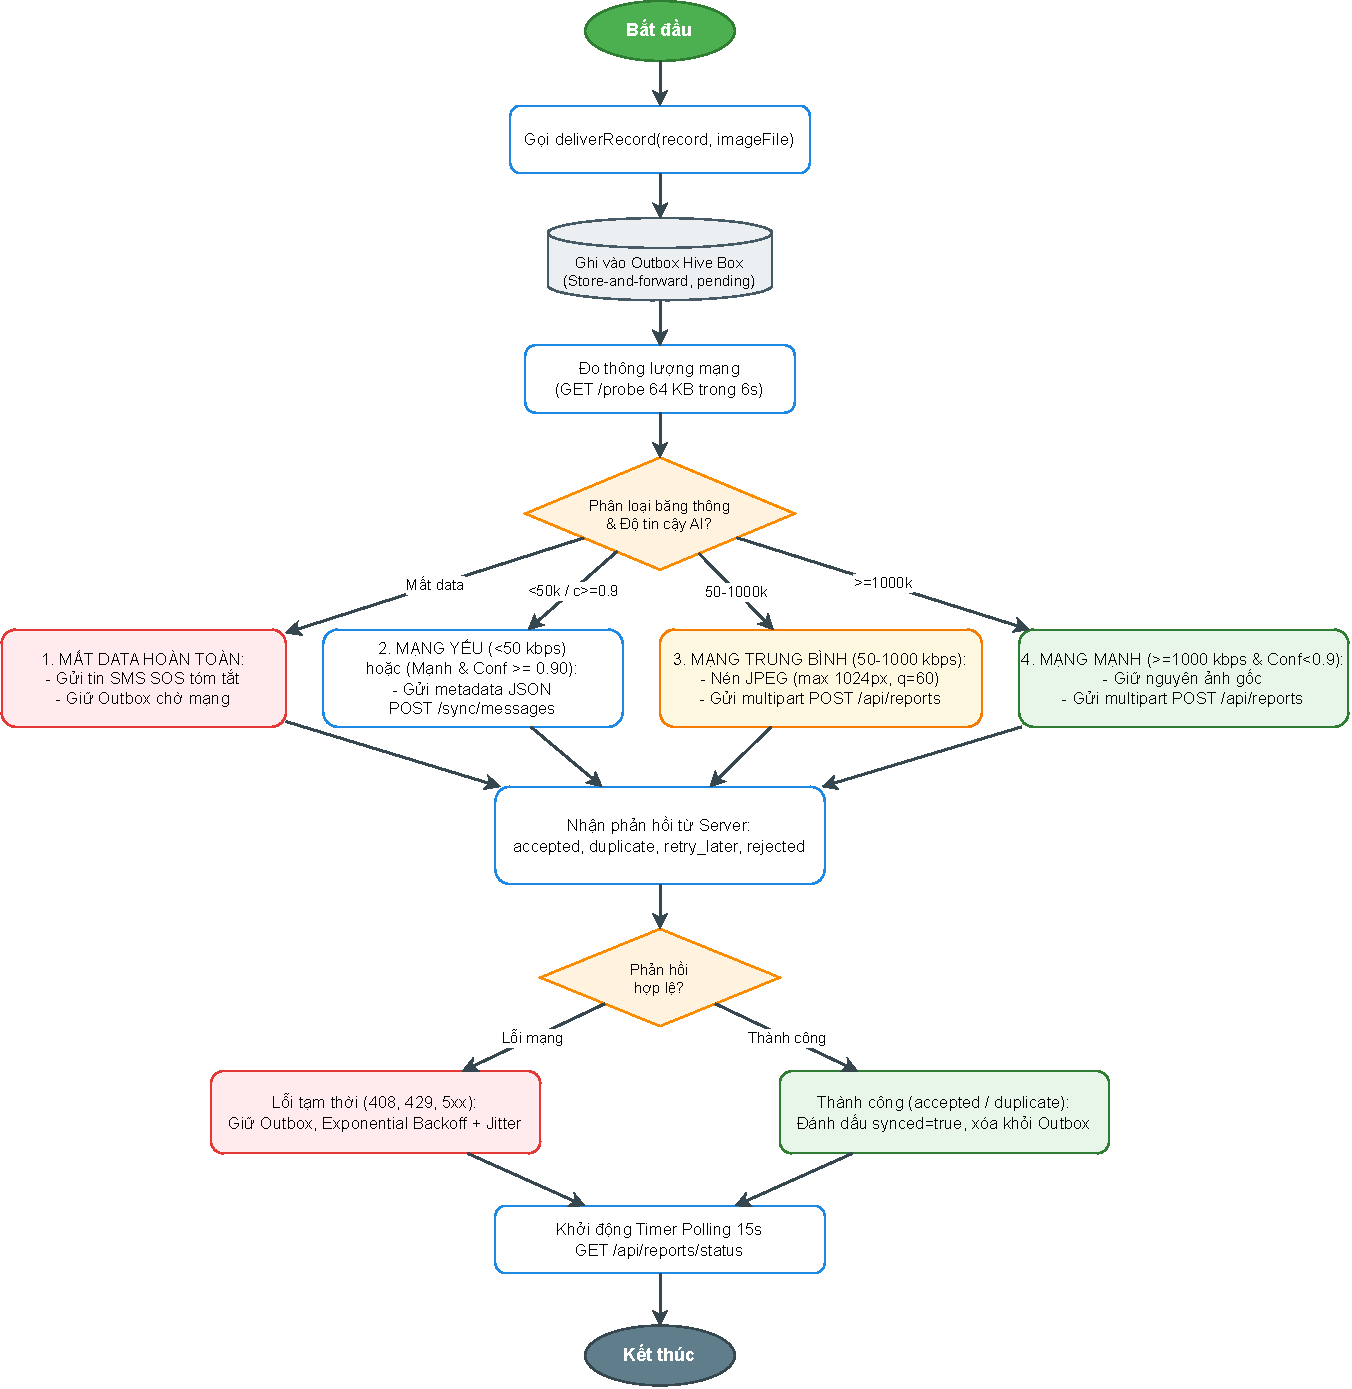
\includegraphics[width=\linewidth,height=\ReportLandscapeImageHeight,keepaspectratio]{flow_03_adaptive_network_send.pdf}
\caption{Lưu đồ quyết định chế độ gửi thích ứng theo thông lượng mạng và độ tin cậy AI}
\label{fig:flow-adaptive-send}
\end{reportlandscapefigure}

